\chapter{DÜŞÜK GÜÇ ANALİZİ VE YENİ ANAHTARLAMA YÖNTEMİ}
\label{chap:anahtarlama}

T-tipi dönüştürücünün düşük güç bölgesindeki davranışı, yalnızca aktarılan aktif gücün azalmasıyla açıklanamaz. Modülasyon indeksinin küçülmesi aktif gerilim durumlarının süresini azaltırken sıfır durumunun ve nötr kol üzerinden gerçekleşen serbest dolaşımın payını artırır. Endüktör akımı bir anahtarlama periyodu içinde sıfıra ulaştığında klasik senkron anahtarlama ters yönde akıma izin verebilir. Yararlı çıkış gücüne katkı sağlamayan ters akım, yarı iletkenlerin ve filtre elemanlarının RMS akımını artırarak hafif yük verimini düşürür. Ters akım yolunun kesilmesi ise süreksiz iletime ve akım dalga biçiminde özellikle üçüncü harmonik bileşenin büyümesine neden olabilir. Dolayısıyla düşük güçteki temel tasarım problemi, verim artışı ile harmonik performans arasındaki ödünleşimin yönetilmesidir.

Bölüm~\ref{chap:sistem} altında T-tipi faz kolunun gerilim durumları, akım yolları ve LCL filtre modeli tanımlanmıştır. Mevcut bölümde aynı fiziksel model kullanılarak ters akımın oluşumu incelenmekte, klasik anahtarlama ile önerilen nötr anahtar susturma yöntemi karşılaştırılmakta ve önceki çalışmadan kurtarılan üç benzetim senaryosu kanıt düzeyleri açıkça belirtilerek değerlendirilmektedir.

\eskitezetiketi\ Eski Bölüm~3.6, düşük güç bölgesini yalnız laboratuvar için seçilmiş bir test noktası olarak değil, fotovoltaik eviricilerde gün doğumu ve gün batımı çevresinde; enerji depolama sistemlerinde ise düşük akımlı şarj veya deşarj komutlarında ortaya çıkan gerçek bir işletme koşulu olarak tanımlamaktadır. Fotovoltaik üretim profilleri ile saha ölçümlerinde kısmi yük süresinin ve düşük akımdaki THD artışının gösterilmesi söz konusu işletme gerekçesini desteklemektedir \citep{Mondol2007,AbRahman2020,Chicco2009}. Enerji depolama uygulamalarında çift yönlü güç komutunun geniş bir aralıkta değişebilmesi de dönüştürücünün yalnız anma noktasında değerlendirilmemesini gerektirir \citep{Aneke2016}.

\section{Ters Akım Dolaşım Mekanizması}

Şebekeye verilen faz akımının temel bileşeni $i_g(t)=\hat I_g\sin(\omega_0t)$ olarak ele alınsın. Düşük güçte $\hat I_g$ küçülürken anahtarlama dalgalanmasının genliği aynı oranda küçülmeyebilir. Bölüm~\ref{chap:sistem} içinde verilen sınır koşuluna göre ortalama endüktör akımının dalgalanmanın yarısından küçük olması, akımın anahtarlama periyodu içerisinde sıfırı geçebilmesine yol açar. Klasik diyotlu alçaltıcı dönüştürücüde akım sıfıra ulaştığında serbest dolaşım diyodu doğal olarak kesime gider. Senkron yapıda diyoda paralel anahtar iletimde tutulduğu için aynı doğal kesim gerçekleşmez \citep{Erickson2001,Chen2010}.

T-tipi faz kolunun nötr durumu, pozitif ve negatif yarım periyotlarda senkron alçaltıcı dönüştürücünün serbest dolaşım durumuna benzer bir görev üstlenir. Faz akımı referans yönünde azalarak sıfıra ulaştığında nötr kol iletimde kalırsa LCL filtre kapasitöründe ve şebeke eşdeğerinde bulunan enerji ters yönde akım oluşturabilir. Akımın işaret değiştirdiği söz konusu aralıkta enerji şebekeden veya filtre kapasitöründen nötr noktaya doğru taşınır. Aktarılan ortalama aktif gücü artırmayan dolaşım akımı, iletim ve bakır kayıpları açısından ek yük oluşturur.

Genel senkron-buck dönüştürücüde diyot benzetimi ile zorlanmış sürekli iletimin farkı Bölüm~2'de Şekil~\ref{fig:de-ccm-akim} üzerinde birincil kaynakla gösterilmiştir. Önceki tezin Şekil~3.11--3.12 altında verdiği sürekli ve süreksiz akım şemaları da aynı kuramsal zincirde Şekil~\ref{fig:onceki-tez-ccm-ters-akim} ve Şekil~\ref{fig:onceki-tez-dcm-akim} olarak korunmuştur. Mevcut bölüm, genel hafif-yük davranışını T-tipi faz kolunun nötr durumuna ve ölçülebilir ters akım yüküne uyarlamaktadır \citep{Erickson2001,Mohan2003,Chen2010}.

\eskitezetiketi\ Önceki tez, klasik senkron buck dönüştürücülerde tamamlayıcı sürmenin MOSFET kanalı üzerinden diyot kaybını azaltabildiğini; incelenen T-tipi yapının nötr kolunda ise IGBT kullanılması nedeniyle aynı kazancın daha sınırlı kalabileceğini vurgulamaktadır. Nötr IGBT'lerin iki yönlü akımı sürdürmesiyle oluşan ters dolaşım, düşük güçte tamamlayıcı sürmenin olası iletim avantajını aşan bir kayıp mekanizmasına dönüşebilir. Kesin kayıp karşılaştırması için IGBT ve diyot iletim karakteristikleriyle anahtarlama kayıplarının gerçek parça kodları üzerinden hesaplanması gerekmektedir.

Bir temel periyot $T_0$, faz kolu endüktör akımı $i_L(t)$, istenen enerji aktarım yönünü veren akım referansı $i^{\ast}(t)$ ve işaret fonksiyonu $\operatorname{sgn}(\cdot)$ ile gösterilsin. Referans yönüne ters akımın akım--zaman büyüklüğünü veren ters akım yükü $Q_{\mathrm{rev}}$
\begin{equation}
  Q_{\mathrm{rev}}=\int_0^{T_0}\max\!\left[-i_L(t)\,\operatorname{sgn}\!\left(i^{\ast}(t)\right),0\right]\,\mathrm{d}t
  \label{eq:ters-akim-yuku}
\end{equation}
ile tanımlanabilir. Eşitlik~\eqref{eq:ters-akim-yuku} akımın mutlak yönü yerine referansa göre ters bileşeni seçer ve amper--saniye birimindedir; tek başına kayıp enerjisi veya gücü vermez. Farklı anahtarlama yöntemlerindeki dolaşımı karşılaştırmak için kullanılabilir. Parçalı doğrusal yarı iletken modelinde sabit iletim gerilimi $V_{\mathrm{on}}$, eğim direnci $R_{\mathrm{on}}$, iletimdeki mutlak akım ortalaması $I_{\mathrm{avg,abs}}$ ve RMS akım $I_{\mathrm{rms}}$ ile basitleştirilmiş iletim kaybı
\begin{equation}
  P_{\mathrm{cond}}\simeq V_{\mathrm{on}} I_{\mathrm{avg,abs}}+R_{\mathrm{on}}I_{\mathrm{rms}}^2
  \label{eq:iletim-kaybi-yaklasik}
\end{equation}
ile yaklaştırılabilir \citep{Chen2010,Schweizer2013}. Eşitlik~\eqref{eq:iletim-kaybi-yaklasik} anahtarlama enerjisini ve sıcaklık bağımlılığı içermeyen ilk mertebe bir iletim modelidir. Ortalama aktif gücü değiştirmeyen bir ters akım bile $I_{\mathrm{rms}}$ değerini ve kaybı büyütebilir. Nötr kol anahtarları, filtre endüktansları ve bağlantı iletkenleri aynı RMS artışından etkilenir.

\eskitezetiketi\ Eski Bölüm~3.6.3'te vurgulanan kayıp dağılımı değişimi Eşitlik~\eqref{eq:iletim-kaybi-yaklasik} üzerinden daha açık yorumlanabilir. Düşük akımda $V_{\mathrm{on}}I_{\mathrm{avg,abs}}$ teriminin aktarılan çıkış gücüne oranı büyüdüğünden, yüksek güçte ikincil kalan sabit iletim gerilimi düşümü hafif yük veriminde belirginleşebilir. Modülasyon indeksi küçüldükçe ana güç anahtarlarının aktif durum payı azalırken nötr durumda geçirilen sürenin artması, toplam kaybın ana anahtarlardan nötr kol elemanlarına ve serbest dolaşım yollarına doğru yeniden dağılmasına yol açabilir. Sayısal dağılım henüz sonuç olarak verilmemiştir; anahtar başına iletim süresi, RMS akım, gerçek $V_{\mathrm{CE(sat)}}$/diyot karakteristiği ve geçiş enerjileri kesin model veya parça kodları üzerinden hesaplanacaktır \citep{Schweizer2013,Wang2020,Chen2010}.

Ters akımın yalnız akım işaretine bakılarak belirlenmesi yeterli değildir. Ölçüm gürültüsü, akım sensörü ofseti, PWM güncelleme gecikmesi, ölü zaman ve anahtarlama anındaki diyot iletimi sıfır geçiş çevresinde yanlış karar üretebilir. Güvenilir uygulama; akım eşiği, histerezis, minimum bekleme süresi ve güvenli komütasyon koşullarını birlikte kullanmalıdır. Gerçek kapı kodu bulunmadığı için söz konusu değerler tezde sayısal olarak varsayılmamış, doğrulama gerektiren tasarım değişkenleri olarak bırakılmıştır.

\eskitezetiketi\ Eski Bölüm~3.5.3 ve 3.6.2, akım denetleyicisinin özellikle sıfır geçiş çevresinde referans--ölçüm farkını azaltmak için oluşturduğu düzeltmelerin ana güç anahtarları ile nötr kol arasındaki geçiş sayısını artırabileceğini bildirmektedir. Ham denetleyici kodu bulunmadığından ilgili gözlem doğrulanmış bir kayıp sonucu olarak kabul edilmemiştir. Yeni doğrulamada kapı başına $N_{\mathrm{sw},j}$ geçiş sayısı, kontrol eforu ve ters akım alanı aynı analiz penceresinde birlikte ölçülecek; verim değişiminin ters dolaşımdan mı, ek anahtarlamadan mı yoksa iki etkiden birlikte mi kaynaklandığı Eşitlik~\eqref{eq:ters-akim-anahtarlama-olcutleri} üzerinden sınanacaktır. Ölü zaman ve düşük akımdaki doğrusal olmayan gerilim hatası da aynı değerlendirmede ayrı tutulacaktır \citep{Teodorescu2006PR,Zhang2014Deadtime}.

\section{Senkron Buck Eşdeğer Modeli}

Pozitif yarım periyotta faz kolu $P$ ve $O$, negatif yarım periyotta $N$ ve $O$ durumları arasında anahtarlanır. Her yarım periyot kendi işaretine göre ele alındığında yapı iki senkron buck dönüştürücünün simetrik birleşimi olarak yorumlanabilir \citep{Mohan2003,Erickson2001,Holmes2003}. Ortalama akım ile akım dalgalanması arasındaki ilişki üç çalışma bölgesi oluşturur:

\begin{enumerate}
  \item \textbf{Sürekli iletim bölgesi:} $|\bar i_L|>\Delta i_L/2$ koşulunda akım bir anahtarlama periyodu içinde sıfıra ulaşmaz. Senkron nötr anahtarın iletim gerilim düşümünü azaltması verim açısından yararlıdır.
  \item \textbf{Sınır iletim bölgesi:} $|\bar i_L|\simeq\Delta i_L/2$ noktasında akım periyot sonunda sıfıra yaklaşır. Parametre belirsizlikleri ve gecikmeler nedeniyle yöntem geçişi için histerezis gereklidir.
  \item \textbf{Zorlanmış sürekli iletim bölgesi:} $|\bar i_L|<\Delta i_L/2$ olmasına rağmen senkron anahtarlama sürdürülürse akım sıfırın ötesine geçer. Ters akım kaybı belirginleşirken akımın sürekliliği harmonik performansı destekleyebilir.
\end{enumerate}

Sınır akımı yaklaşık olarak
\begin{equation}
  I_{\mathrm{B}}(t)=\frac{\Delta i_L(t)}{2}
  \label{eq:sinir-akimi}
\end{equation}
şeklinde tanımlanabilir. Eşitlik~\eqref{eq:sinir-akimi} içindeki $I_{\mathrm{B}}$; DA bara gerilimi, anlık şebeke gerilimi, görev oranı, anahtarlama frekansı ve eşdeğer endüktansa bağlıdır. Sabit bir yüzde güç eşiği yerine fiziksel değişkenlerden türetilen sınır akımının kullanılması, şebeke gerilimi veya DA bara seviyesi değiştiğinde daha tutarlı bir kip geçişi sağlayabilir. Filtre değerlerinin ham tasarım kaydı bulunmadığından tezde nihai $I_{\mathrm{B}}$ sayısı verilmemiştir.

\eskitezetiketi\ Senkron-buck eşdeğerinin sağladığı temel avantaj, üç fazlı sistemdeki düşük güç davranışını faz kolu düzeyinde enerji aktarımı, serbest dolaşım ve akım sürekliliği bakımından ayrıştırabilmesidir. Pozitif yarım periyotta üst ana anahtar ile nötr kolun, negatif yarım periyotta ise alt ana anahtar ile karşı nötr yolun görevleri aynı devre modeli üzerinde izlenebilir. Eşdeğer model böylece modülasyon indeksinin küçülmesiyle nötr durum payının artmasını, endüktör akımının sıfırı geçmesini ve hangi kapı geçişlerinin ek anahtarlama yükü oluşturduğunu ortak bir fiziksel çerçeveye bağlamaktadır. Yaklaşım yalnız kavramsal benzetme olarak kullanılmamış; sınır akımı, ters akım alanı ve anahtar geçiş sayısı ölçütlerinin kurulmasına temel oluşturmuştur.

\section{Klasik Anahtarlama Yöntemi}

Klasik üç seviyeli modülasyonda nötr kol, sıfır gerilim durumunu üretmek üzere her iki yarım periyotta etkin kullanılır. Pozitif alternansta aktif enerji aktarımı $P$ durumu, serbest dolaşım $O$ durumu; negatif alternansta aktif enerji aktarımı $N$ durumu, serbest dolaşım yine $O$ durumu üzerinden gerçekleşir. Akım referansı küçüldüğünde aktif durumun görev oranı azalır ve nötr durumda geçirilen süre uzar.

\eskitezetiketi\ Önceki benzetim kurgusunda üç fazlı, dört telli yapının her fazı bağımsız bir tek fazlı T-tipi kol olarak ele alınmış ve kapı işaretleri sinüzoidal PWM ile üretilmiştir. Faz başına inceleme, nötr anahtar müdahalesinin hangi yarım periyotta ve hangi kol üzerinde yapıldığını açıkça göstermektedir. Yöntemin uzay vektör PWM veya başka modülasyon tekniklerine genellenmesi ise mevcut kanıtın dışında kalan ayrı bir doğrulama konusudur.

Senkron anahtarlamanın temel üstünlüğü, normal ve yüksek akım bölgesinde diyot iletimini düşük gerilim düşümlü anahtar kanalıyla değiştirebilmesidir. Aynı davranış düşük güçte nötr kolun akımı iki yönde de iletebilmesi nedeniyle dezavantaja dönüşür. Akım sıfıra ulaştıktan sonra kapı komutunun korunması, akım yönünü sınırlayan doğal bir diyot kesimi bırakmaz. Sonuç olarak klasik yöntem düşük THD sağlayabilmesine karşın hafif yükte ters akım alanı ve RMS akım bakımından elverişsiz olabilir.

\begin{table}[htbp]
  \centering
  \caption{\eskitezetiketi\ \juriistegietiketi\ Klasik ve önerilen anahtarlamanın düşük güçte işlevsel karşılaştırması.}
  \label{tab:klasik-onerilen-islevsel}
  \small
  \begin{tabularx}{\textwidth}{p{0.22\textwidth} X X}
    \toprule
    Özellik & Klasik senkron anahtarlama & Önerilen nötr anahtar susturma \\
    \midrule
    Sıfır durumu & Nötr kol iki yönlü akıma izin verir. & Ters dolaşıma yol açan nötr komutu düşük güç bölgesinde engellenir. \\
    Akım sürekliliği & Sıfır geçişten sonra ters yönde sürdürülebilir. & Akım sıfırda doğal olarak kesilebilir; süreksiz iletim oluşabilir. \\
    Beklenen kayıp etkisi & Ters akım nedeniyle RMS ve iletim kaybı artabilir. & Ters akım yolu azaltıldığı için iletim kaybı düşebilir. \\
    Beklenen harmonik etkisi & Akım sürekliliği THD açısından avantaj sağlayabilir. & Üçüncü harmonik ve THD belirgin biçimde artabilir. \\
    Gerekli tamamlayıcı önlem & Özel düşük güç müdahalesi yoktur. & Sin\textsuperscript{3} kompanzasyonu ve güvenli kip geçişi gerekir. \\
    \bottomrule
  \end{tabularx}
\end{table}

\begin{center}
\juriistegietiketi\ \small Jürinin T-tipi çalışma modlarının açıklanması talebi doğrultusunda anahtarlama farkı; akım yolu, kayıp etkisi ve harmonik sonucu aynı karşılaştırma altında verilmiştir.
\end{center}

\section{Önerilen Anahtarlama Yöntemi}

Önerilen yöntemin amacı, düşük güçte referans enerji yönüne ters akımı sürdüren nötr anahtar komutunu bastırmaktır. Yöntem klasik PWM yapısını tüm çalışma aralığında değiştirmemekte, yalnız akımın sınır iletim bölgesine yaklaştığı koşullarda devreye girmektedir. Yarım periyot işareti, akım referansı ve ölçülen akım birlikte değerlendirilerek yararlı akım yönünün tersine iletime yol açan nötr komut belirlenir.

İkili etkinleştirme değişkeni $\sigma(t)\in\{0,1\}$, düşük güç geçiş eşiği $I_{\mathrm{th}}$, pozitif histerezis genişliği $H$ ve ters iletim koşulunu gösteren ikili gösterge $\chi_{\mathrm{rev}}(t)\in\{0,1\}$ ile tanımlansın. Histerezis bandında önceki durumun korunmasını da içeren işlevsel kural
\begin{equation}
  \sigma(t)=
  \begin{cases}
    1, & |i^{\ast}(t)|\leq I_{\mathrm{th}}\ \text{ve }\chi_{\mathrm{rev}}(t)=1,\\
    0, & |i^{\ast}(t)|\geq I_{\mathrm{th}}+H\ \text{veya }\chi_{\mathrm{rev}}(t)=0,\\
    \sigma(t^-), & I_{\mathrm{th}}<|i^{\ast}(t)|<I_{\mathrm{th}}+H\ \text{ve }\chi_{\mathrm{rev}}(t)=1
  \end{cases}
  \label{eq:susturma-etkinlestirme}
\end{equation}
ile gösterilebilir. Eşitlik~\eqref{eq:susturma-etkinlestirme} içindeki $t^-$ karar anından hemen önceki durumu gösterir; böylece iki satırlı eski tanımda boş kalan histerezis aralığı kapatılmıştır. Klasik ve yeni nötr kapı komutları $g_{n,\mathrm{kl}}(t)$ ile $g_{n,\mathrm{yeni}}(t)$ olarak tanımlandığında
\begin{equation}
  g_{n,\mathrm{yeni}}(t)=g_{n,\mathrm{kl}}(t)\left[1-\sigma(t)\chi_{\mathrm{rev}}(t)\right]
  \label{eq:notr-susturma-kurali}
\end{equation}
biçiminde özetlenebilir. Denklem~\eqref{eq:notr-susturma-kurali} gerçek sürücüye doğrudan aktarılacak kesin bir kapı tablosu değil, yöntemin hangi komutu hangi amaçla değiştirdiğini belirleyen işlevsel tanımdır. Anahtarların gerçek adları, polariteleri ve güvenli komütasyon sırası kaynak kod veya sürücü kaydı bulunmadan kesinleştirilemez.

Önceki tezde klasik ve nötr anahtar susturmalı yöntemler için hem tam temel periyot hem de seçilmiş anahtarlama penceresinin yakın görünümü verilmiştir. Görseller aynı içeriğin tekrarı değildir: eski Şekil 4.1 ve 4.2 klasik anahtarlamayı, eski Şekil 4.10 ve 4.11 ise nötr anahtar susturmalı yöntemi göstermektedir. İzlenebilirliği korumak için dört kayıt yeni tezde de birleştirilmeden ayrı şekiller olarak kullanılmıştır. Klasik yöntem Şekil~\ref{fig:klasik-kapi-darbeleri-tam} ve Şekil~\ref{fig:klasik-kapi-darbeleri-yakin}, önerilen yöntem ise Şekil~\ref{fig:susturma-kapi-darbeleri-tam} ve Şekil~\ref{fig:susturma-kapi-darbeleri-yakin} altında verilmektedir.

\begin{figure}[htbp]
  \centering
  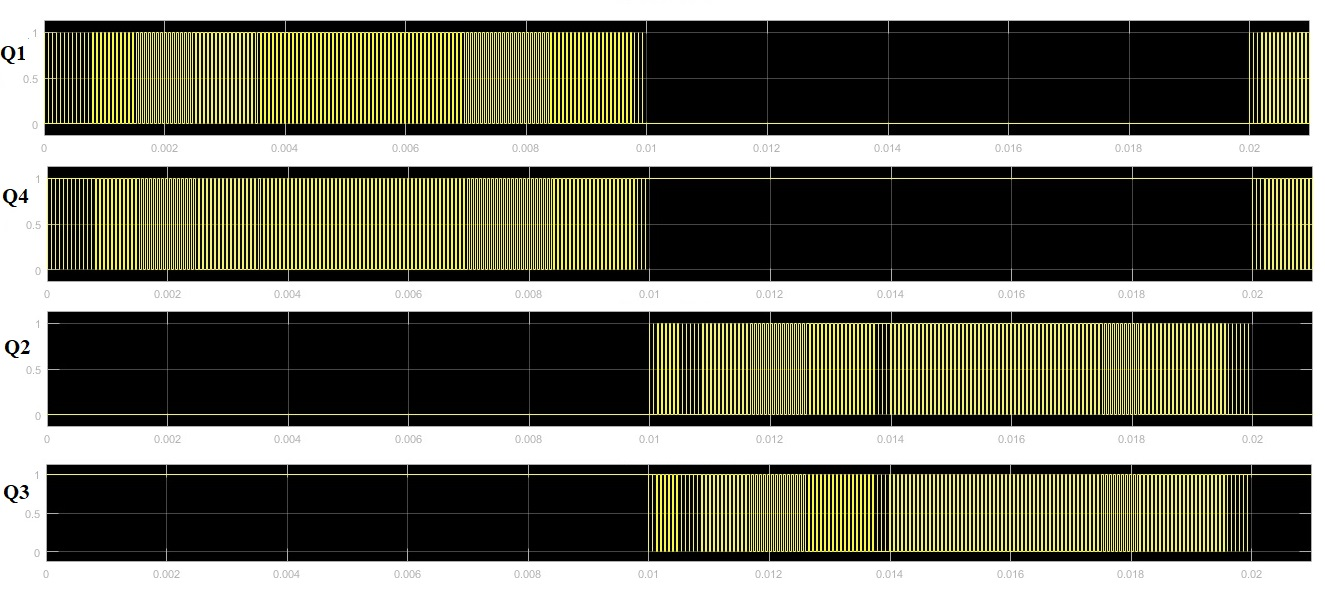
\includegraphics[width=0.98\textwidth]{sistem/onceki_tez_klasik_kapi_darbeleri.jpg}
  \caption{\eskitezetiketi\ Klasik tamamlayıcı anahtarlamada $Q_1$--$Q_4$ kapı darbelerinin bir temel periyot boyunca görünümü (eski Şekil 4.1).}
  \label{fig:klasik-kapi-darbeleri-tam}
\end{figure}

\begin{figure}[H]
  \centering
  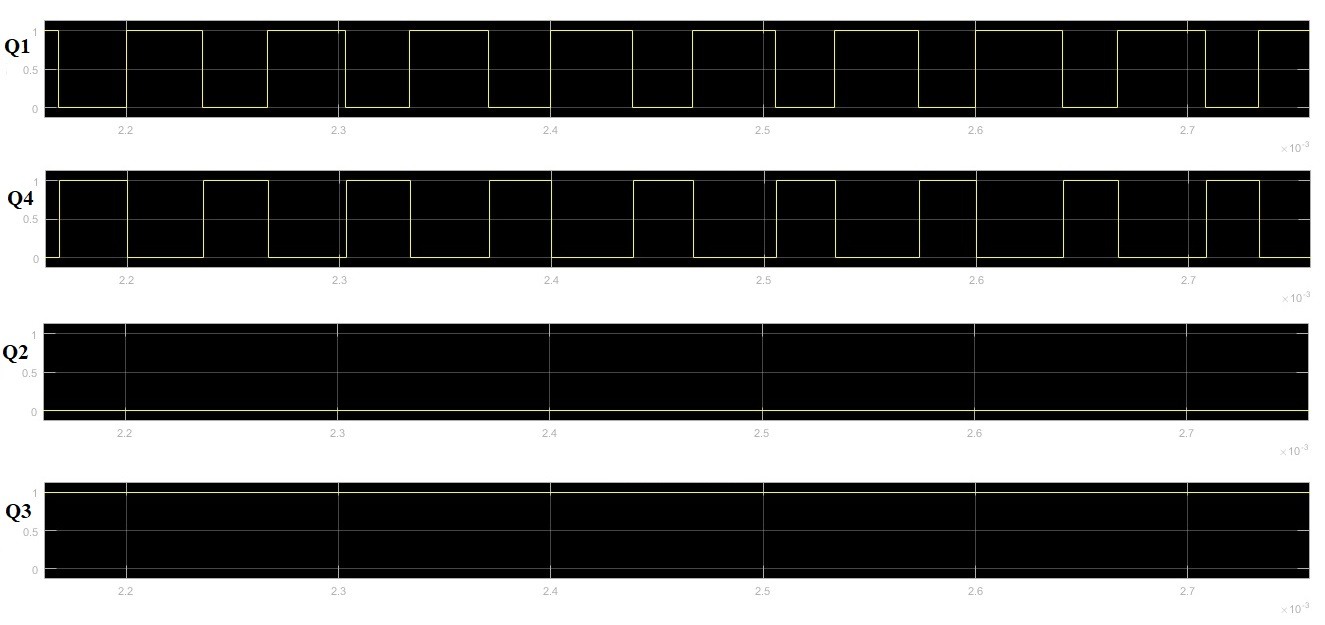
\includegraphics[width=0.98\textwidth]{sistem/onceki_tez_klasik_kapi_darbeleri_yakin.jpg}
  \caption{\eskitezetiketi\ Klasik tamamlayıcı anahtarlamada seçilmiş anahtarlama penceresinin yakın görünümü (eski Şekil 4.2).}
  \label{fig:klasik-kapi-darbeleri-yakin}
\end{figure}

Şekil~\ref{fig:klasik-kapi-darbeleri-yakin} altındaki pozitif alternans kesitinde $Q_1$ ile $Q_4$ tamamlayıcı darbelerle anahtarlanırken $Q_2$ kesimde, $Q_3$ iletimde tutulmaktadır. Aynı zaman aralığında önerilen yöntemi gösteren Şekil~\ref{fig:susturma-kapi-darbeleri-yakin} altında $Q_1$ anahtarlamayı sürdürmekte, nötr kola ait $Q_4$ komutu ise sıfırda tutulmaktadır. Önceki tez, simetrik olarak negatif alternansta $Q_3$ komutunun bastırıldığını bildirmektedir. Yakın görünümler tam periyot şekillerinin tekrarı değil, kapılar arasındaki darbe ilişkisini anahtarlama periyodu ölçeğinde gösteren ayrı kayıtlardır. Ekran kayıtları ölü zamanı, minimum darbe genişliğini, lojik polariteyi ve sürücü gecikmesini doğrulayamadığından kesin kapı tablosu gerçek PWM koduyla kilitlenecektir.

Eski benzetim modelinin faz kolu ve tüm sistem ekranı da sonuç dalga biçimlerinden ayrı kanıt türleridir. Şekil~\ref{fig:onceki-faz-modeli}, $Q_1$--$Q_4$, bölünmüş DA bara, $L_1$, $C_1$ ve $L_2$ elemanlarının kullanılan tek fazlı T-tipi kola nasıl bağlandığını göstermektedir. Şekil~\ref{fig:onceki-simulasyon-modeli} ise ölçüm, filtre, şebeke eşdeğeri ve güç hesabı bloklarını içeren üst düzey Simulink çalışma alanını belgelemektedir. Sonradan gelen Senaryo~1 `.slx` dosyası bu genel yapıyla uyumludur; ancak R2025b'de kaldırılan ölçüm blokları ve Senaryo~2--3 model/kodlarının yokluğu nedeniyle ekranlar üç senaryonun yeniden üretilebilir ortak model kanıtı değildir.

\begin{figure}[H]
  \centering
  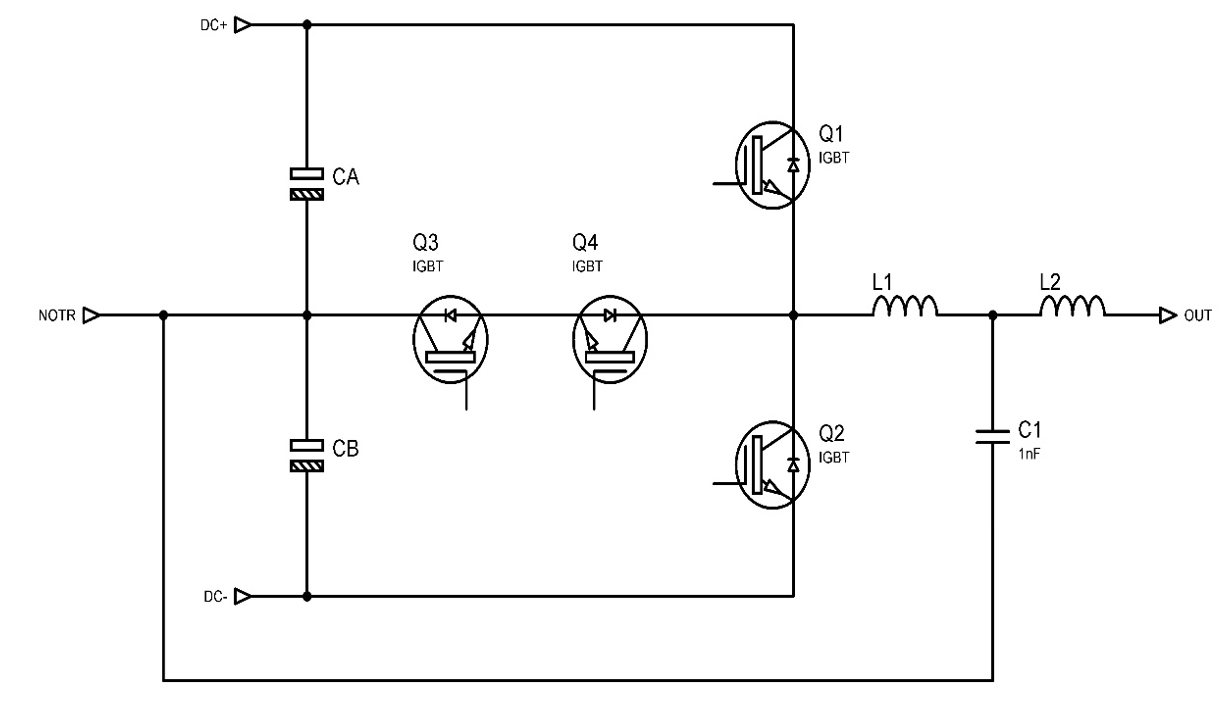
\includegraphics[width=0.90\textwidth]{sonuclar/onceki_tez_t_tipi_faz_modeli.png}
  \caption{\eskitezetiketi\ Önceki benzetimde kullanılan tek fazlı T-tipi evirici ve LC filtre yapısı (eski Şekil 4.3).}
  \label{fig:onceki-faz-modeli}
\end{figure}

\begin{figure}[H]
  \centering
  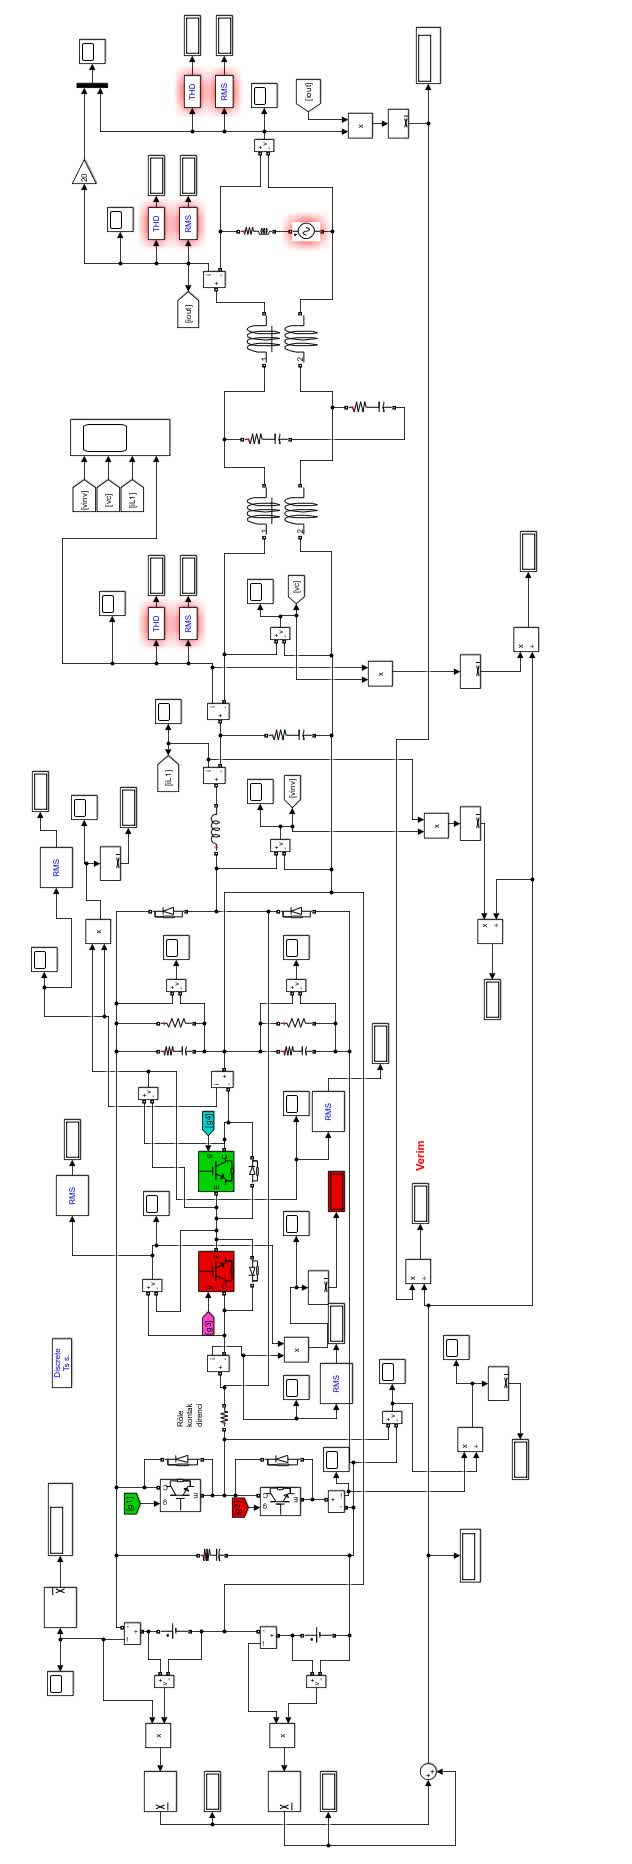
\includegraphics[angle=90,width=0.96\textwidth]{sonuclar/onceki_tez_simulasyon_modeli.jpg}
  \caption{\eskitezetiketi\ Önceki çalışmada kullanılan Simulink modelinin genel görünümü (eski Şekil 4.4). Sonradan gelen Senaryo~1 modeliyle yapısal olarak karşılaştırılmış, üç senaryonun ortak koşulu olarak doğrulanmamıştır.}
  \label{fig:onceki-simulasyon-modeli}
\end{figure}

Güvenli uygulamada dört koşul birlikte sağlanmalıdır. İlk olarak, akım işareti sensör ofsetinden büyük bir güven payıyla belirlenmelidir. İkinci olarak, nötr kolun kesilmesi endüktör akımı için kesintisiz ve aşırı gerilim üretmeyen alternatif bir yol bırakmalıdır. Üçüncü olarak, karşılıklı anahtarların ölü zamanı ve minimum darbe genişliği korunmalıdır. Son olarak, ölçüm geçersizliği veya aşırı akım durumunda denetim önceden tanımlanmış güvenli anahtarlamaya dönmelidir. Ölü zaman içermeyen aday benzetim parametre dosyası ilk yeniden üretim koşulunu göstermekte; gerçek donanım için ölü zaman ve sürücü gecikmesi ayrıca doğrulanmalıdır \citep{Zhang2014Deadtime}.

Nötr anahtarın bastırılması ters akım yolunu azaltırken endüktör akımını süreksiz iletime zorlar. Akımın sıfır çevresindeki düzleşmesi ve iletim aralıklarının daralması, temel bileşene göre üçüncü harmonik payını büyütür. Dolayısıyla önerilen anahtarlama tek başına nihai yöntem değildir; Bölüm~\ref{chap:sin3} altında incelenen Sin\textsuperscript{3} ileri besleme kompanzasyonu, ortaya çıkan harmonik cezanın azaltılması için tamamlayıcı katman olarak kullanılmaktadır.

\eskitezetiketi\ Önceki tezdeki mekanizma açıklaması, nötr susturma sonrasında faz kolunu pozitif ve negatif alternanslar için iki buck dönüştürücü gibi ele almaktadır. Süreksiz iletimde akım zarfı, görev oranı ile anahtarlama anındaki endüktör gerilim farkının birlikte değişmesi nedeniyle saf sinüs biçimini koruyamaz. Alternans ortasında, yaklaşık $\omega_0t=\pi/2$ ve $3\pi/2$ çevresinde, DA bara ile şebeke gerilimi arasındaki akım yükseltme payının azalması akım zarfında çökme oluşturabilir; sıfır geçişlerine yakın bölgelerdeki farklı yükselme hızı da üçüncü harmonik bileşeni besler. Parçalı DCM--CCM denklemleri, kritik görev oranı ve Sin\textsuperscript{3} katsayı taraması, doğrulanmış devre parametreleriyle Bölüm~\ref{chap:sin3} altında yeniden kurulacaktır.

\tezcalismanotu{D4-1 --- Kapı mantığı ve senaryo eşlemesinin kodla kesinleştirilmesi}{Senaryo~1 modeli alınmış; modelde klasik kapı üretimi görülebilmiş, ancak R2025b sürüm uyumsuzluğu nedeniyle kaynak koşu tamamlanamamıştır. Senaryo~2--3 PWM modeli veya kontrol kodu bulunmadığından pozitif alternansta $Q_4$, negatif alternansta $Q_3$ susturma kuralı kesin kod doğrulaması değildir. Dönüştürülmüş ortak modelde $Q_1$--$Q_4$ doğruluk tablosu, tamamlayıcılık, ölü zaman, akım işareti, eşik/histerezis ve kip geçişleri yeniden çıkarılacaktır.}

\section{Verim ve Harmonik Performans Ödünleşimi}

Sonradan ulaştırılan üç senaryo arşivi aynı düşük güç probleminin ardışık karşılaştırma kolları olarak değerlendirilmiştir. Dalga biçimleri ve eski teknik açıklama birlikte incelendiğinde Senaryo~1 klasik senkron anahtarlama, Senaryo~2 nötr anahtar susturma, Senaryo~3 ise susturma ile Sin\textsuperscript{3} kompanzasyonunun birlikte kullanımıyla yüksek ölçüde uyumludur. Yalnız Senaryo~1 için kaynak `.slx` gelmiş, Senaryo~2--3 kapı kodu gelmemiştir; bu nedenle eşleme ``yüksek güvenli'' düzeyde tutulmuş, kesin kod doğrulaması olarak sunulmamıştır.

\eskitezetiketi\ Eski Bölüm 4'teki benzetim açıklaması; üç fazlı dört telli sistemin faz başına modellenmesini, üst güç sınıfı çalışma kaydının “\SI{25}{\kilo\watt}” olarak adlandırılmasını, düşük güç incelemesinin yaklaşık \SI{2.6}{\ampere} RMS faz akımında yapılmasını ve yapısal etkiyi ayırmak için akım denetleyicisinin devre dışı bırakılarak yalnızca ileri besleme katsayısının değiştirilmesini bildirmektedir. Aynı kayıt, uygulamaya benzerlik amacıyla EMC filtre ve varyak gibi bileşenlerin benzetim modeline eklendiğini de belirtmektedir. Model dosyası, bileşen parametreleri ve kayıp tanımları bulunmadığından söz konusu koşullar yeni doğrulama modeli olarak kabul edilmemiştir. Eski metindeki \SI{20}{\kilo\watt}/\SI{25}{\kilo\watt} adlandırması ile yeni sistem tablosundaki \SI{20}{\kilo\volt\ampere} kaydı da ham tasarım belgesi üzerinden kesinleştirilecektir.

FFT ekranlarında analiz başlangıcı \SI{0.06}{\second}, pencere uzunluğu iki temel çevrim ve temel frekans \SI{50}{\hertz} olarak verilmiştir. Görüntüleme üst sınırı \SI{550}{\hertz} olup THD hesabının Nyquist frekansına kadar yürütüldüğü ekran üzerinde belirtilmektedir. Tablo~\ref{tab:senaryo-thd}, ekranlardan doğrudan okunan değerleri aynı ölçüm tanımı altında toplamaktadır.

\begin{table}[htbp]
  \centering
  \caption{\eskitezetiketi\ \juriistegietiketi\ Kurtarılan düşük güç benzetim ekranlarından okunan temel bileşen ve THD değerleri.}
  \label{tab:senaryo-thd}
  \small
  \begin{tabular}{c l S[table-format=1.3] S[table-format=2.2] S[table-format=1.3] S[table-format=2.2]}
    \toprule
    {Senaryo} & {Yöntem eşlemesi} & {$I_{L1,1}$ (A)} & {$\mathrm{THD}_{L1}$ (\%)} & {$I_{\mathrm{out},1}$ (A)} & {$\mathrm{THD}_{\mathrm{out}}$ (\%)} \\
    \midrule
    1 & Klasik anahtarlama & 3.698 & 8.29 & 3.734 & 2.14 \\
    2 & Nötr anahtar susturma & 3.396 & 46.86 & 3.412 & 46.35 \\
    3 & Susturma + Sin\textsuperscript{3} & 3.752 & 9.46 & 3.766 & 7.79 \\
    \bottomrule
  \end{tabular}
\end{table}

Önceki tezde aynı üç yöntem için verim ve THD değerlerini birlikte veren bir benzetim özeti de bulunmaktadır. Tablo~\ref{tab:onceki-benzetim-ozeti}, kayıp hesabının yapıldığı ham model mevcut olmadığından ayrı kanıt statüsüyle aktarılmıştır. THD değerleri kurtarılan FFT ekranlarıyla yakından uyuşurken verim yüzdeleri yeniden hesaplanamamıştır.

\begin{table}[htbp]
  \centering
  \caption{\eskitezetiketi\ Önceki tezde raporlanan benzetim verimi ve akım THD değerleri; verim hesabı ham model beklemektedir.}
  \label{tab:onceki-benzetim-ozeti}
  \begin{tabular}{>{\raggedright\arraybackslash}p{0.43\textwidth}ccc}
    \toprule
    \textbf{Yöntem} & \textbf{Verim (\%)} & \textbf{$\mathrm{THD}_{L1}$ (\%)} & \textbf{$\mathrm{THD}_{faz}$ (\%)} \\
    \midrule
    Klasik tamamlayıcı anahtarlama & 90,45 & 8,30 & 2,10 \\
    Nötr anahtar susturma & 93,00 & 46,90 & 46,30 \\
    Susturma + Sin\textsuperscript{3} & 93,70 & 9,50 & 7,80 \\
    \bottomrule
  \end{tabular}
\end{table}

Senaryo~2'de $I_{L1}$ ve $I_{\mathrm{out}}$ THD değerlerinin sırasıyla \%46,86 ve \%46,35'e çıkması, nötr anahtar susturmanın tek başına oluşturduğu harmonik cezayı göstermektedir. Senaryo~3'te aynı değerlerin \%9,46 ve \%7,79'a gerilemesi, Senaryo~2'ye göre yaklaşık \%79,8 ve \%83,2 bağıl azalma anlamına gelir. Kompanzasyon sonrasında temel akım genliklerinin Senaryo~1 ile yakın seviyeye dönmesi de yöntemin düşük güç akımını bütünüyle bastırmadığını göstermektedir. Yine de Senaryo~3 çıkış THD değeri Senaryo~1'in \%2,14 seviyesine ulaşmamıştır; kompanzasyonun iyileştirici fakat ideal olmayan sonucu açıkça korunmalıdır.

Senaryo~2'nin ayrı kapı, $L_1$ akımı, dört-kanal dalga biçimi ve FFT kayıtları Şekil~\ref{fig:susturma-kapi-darbeleri-tam}--\ref{fig:susturma-iout-fft} altında özgün sıralarıyla verilmiştir. Senaryo~3 ekranı Sin\textsuperscript{3} kompanzasyonunun sonuç setine ait olduğundan Bölüm~\ref{chap:sin3} altında eski Şekil 4.29--4.32 ile birlikte ele alınacaktır. Sayısal yorum yalnız görüntüden okunabilen kanallarla sınırlandırılmıştır; anahtarlama kaybı, yarı iletken sıcaklığı ve DA/AA güçleri kaydedilmediği için üç senaryo arasında doğrudan verim artışı yüzdesi hesaplanamaz.

Sonradan ulaştırılan Senaryo~1 paketi, önceki tezin Şekil 4.5--4.9 altında verdiği klasik anahtarlama sonuçlarının yüksek çözünürlüklü kaynak ekranlarını içermektedir. Eski tez dosyasından çıkarılan tek-kanal kayıtlar ile yeni paketteki dört-kanallı ekranın dalga zarfı ve sayısal FFT sonuçları birbiriyle örtüşmektedir. Dolayısıyla söz konusu beş sonuç aşağıda aynı teknik sırayla korunmuş; ham zaman serisi bulunmadığı için yeniden hesaplanmış benzetim çıktısı yerine kurtarılmış benzetim kanıtı olarak sınıflandırılmıştır.

Şekil~\ref{fig:klasik-l1-tam}, klasik tamamlayıcı anahtarlamada $L_1$ endüktör akımının bir temel periyot içindeki anahtarlama dalgalanmasını göstermektedir. Akım zarfının temel bileşen boyunca değişmesi ve yüksek frekanslı üçgensel dalgalanmanın zarf üzerine binmesi, düşük güçte anlık akımın sıfır çevresine yaklaşabildiğini göstermesi bakımından önemlidir.

\begin{figure}[H]
  \centering
  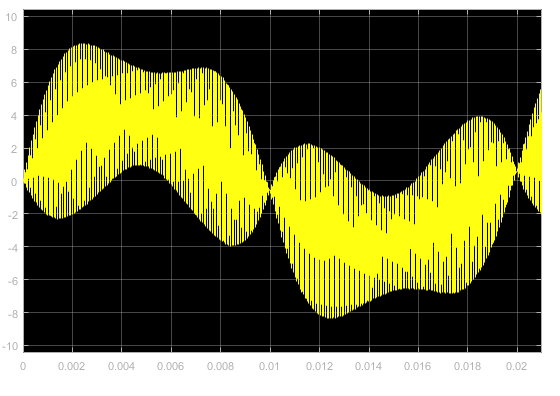
\includegraphics[width=0.82\textwidth]{sonuclar/onceki_tez_l1_tam.png}
  \caption{\eskitezetiketi\ Klasik anahtarlama benzetiminden elde edilen $L_1$ endüktör akımının tam-periyot dalga biçimi (eski Şekil 4.5; Senaryo~1 kaynak ekranıyla doğrulanmıştır).}
  \label{fig:klasik-l1-tam}
\end{figure}

Şekil~\ref{fig:klasik-l1-yakin}, yaklaşık \SI{0.9}{\milli\second}--\SI{1.8}{\milli\second} aralığını büyüterek akım dalgalanmasının anahtarlama periyodu ölçeğindeki yapısını görünür kılmaktadır. Yaklaşık \SI{10}{\kilo\hertz} anahtarlama frekansıyla uyumlu üçgensel değişim, $L_1$ akımındaki dalgalanmanın yalnız düşük frekanslı zarf üzerinden değerlendirilmemesi gerektiğini göstermektedir.

\begin{figure}[!htbp]
  \centering
  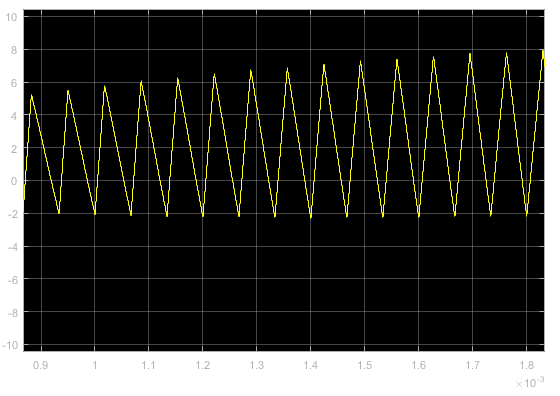
\includegraphics[width=0.82\textwidth]{sonuclar/onceki_tez_l1_yakin_0_9_1_8ms.png}
  \caption{\eskitezetiketi\ Klasik anahtarlama benzetimindeki $L_1$ endüktör akımından büyütülmüş kesit (eski Şekil 4.6).}
  \label{fig:klasik-l1-yakin}
\end{figure}

Senaryo~1'in yüksek çözünürlüklü kaynak ekranı Şekil~\ref{fig:klasik-dort-kanal} altında verilmiştir. Yukarıdan aşağıya kanallar; anahtarlama devresi çıkışındaki filtre giriş gerilimini, LC filtre girişine uygulanan gerilimin filtrelenmiş hâlini, $L_1$ endüktör akımını ve LC filtre çıkış akımını göstermektedir. Önceki tez başlığında ikinci kanal ``kontrolör çıkış işareti'' olarak adlandırılmıştır; sonradan gelen özgün ekran üzerindeki kanal başlığı gerilim işaretini açıkça tanımladığından yeni tezde hatalı adlandırma tekrarlanmamıştır. İlk iki kanal anahtarlama geriliminin filtrelenmesini, son iki kanal ise $L_1$ dalgalanmasının çıkış akımında ne ölçüde bastırıldığını aynı zaman ekseninde izlemeyi sağlamaktadır.

\begin{figure}[H]
  \centering
  \includegraphics[width=0.98\textwidth]{../dosyalar/05_sonradan_gelenler/Senaryo_1/dalga_sekli_s1.jpg}
  \caption{\eskitezetiketi\ Klasik anahtarlamada filtre giriş gerilimi, filtrelenmiş gerilim, $L_1$ endüktör akımı ve LC filtre çıkış akımının birlikte gösterimi (eski Şekil 4.7'nin düzeltilmiş kanal açıklaması).}
  \label{fig:klasik-dort-kanal}
\end{figure}

FFT sonuçları, aynı klasik anahtarlama koşulunda filtrenin akım harmonikleri üzerindeki etkisini iki ölçüm noktasında göstermektedir. Şekil~\ref{fig:klasik-l1-fft} altında $L_1$ akımının temel bileşeni \SI{3.698}{\ampere} ve THD değeri \%8,29; Şekil~\ref{fig:klasik-iout-fft} altında çıkış akımının temel bileşeni \SI{3.734}{\ampere} ve THD değeri \%2,14 olarak okunmaktadır. Analizlerin \SI{0.06}{\second} başlangıçlı iki çevrimlik aynı pencereyi kullanması, iki değerin karşılaştırılabilir olmasını desteklemektedir. Çıkış akımındaki THD'nin $L_1$ akımına göre yaklaşık \%74,2 azalması, LC filtrenin anahtarlama kaynaklı harmonikleri bastırdığını nicel olarak göstermektedir.

\begin{figure}[H]
  \centering
  \includegraphics[width=0.98\textwidth]{../dosyalar/05_sonradan_gelenler/Senaryo_1/THD_IL1.jpg}
  \caption{\eskitezetiketi\ Klasik anahtarlamada $L_1$ endüktör akımının FFT analizi: temel bileşen \SI{3.698}{\ampere}, $\mathrm{THD}_{L1}=\%8{,}29$ (eski Şekil 4.8).}
  \label{fig:klasik-l1-fft}
\end{figure}

\begin{figure}[H]
  \centering
  \includegraphics[width=0.98\textwidth]{../dosyalar/05_sonradan_gelenler/Senaryo_1/THD_Iout.jpg}
  \caption{\eskitezetiketi\ Klasik anahtarlamada LC filtre çıkış akımının FFT analizi: temel bileşen \SI{3.734}{\ampere}, $\mathrm{THD}_{\mathrm{out}}=\%2{,}14$ (eski Şekil 4.9).}
  \label{fig:klasik-iout-fft}
\end{figure}

Nötr anahtar susturma yöntemine ait eski Şekil 4.10--4.16, klasik anahtarlama sonuçlarından farklı yedi görseldir. Şekil~\ref{fig:susturma-kapi-darbeleri-tam} ve Şekil~\ref{fig:susturma-kapi-darbeleri-yakin} kapı komutlarını; Şekil~\ref{fig:susturma-l1-tam} ve Şekil~\ref{fig:susturma-l1-yakin} $L_1$ akımını; Şekil~\ref{fig:susturma-dort-kanal} sistemin dört ölçüm kanalını; Şekil~\ref{fig:susturma-l1-fft} ve Şekil~\ref{fig:susturma-iout-fft} ise iki farklı akım ölçüm noktasının FFT sonuçlarını göstermektedir. Görsellerin ayrı tutulması, anahtarlama müdahalesi ile ortaya çıkan akım ve harmonik sonuçları arasındaki neden--sonuç zincirini izlenebilir kılmaktadır.

\begin{figure}[H]
  \centering
  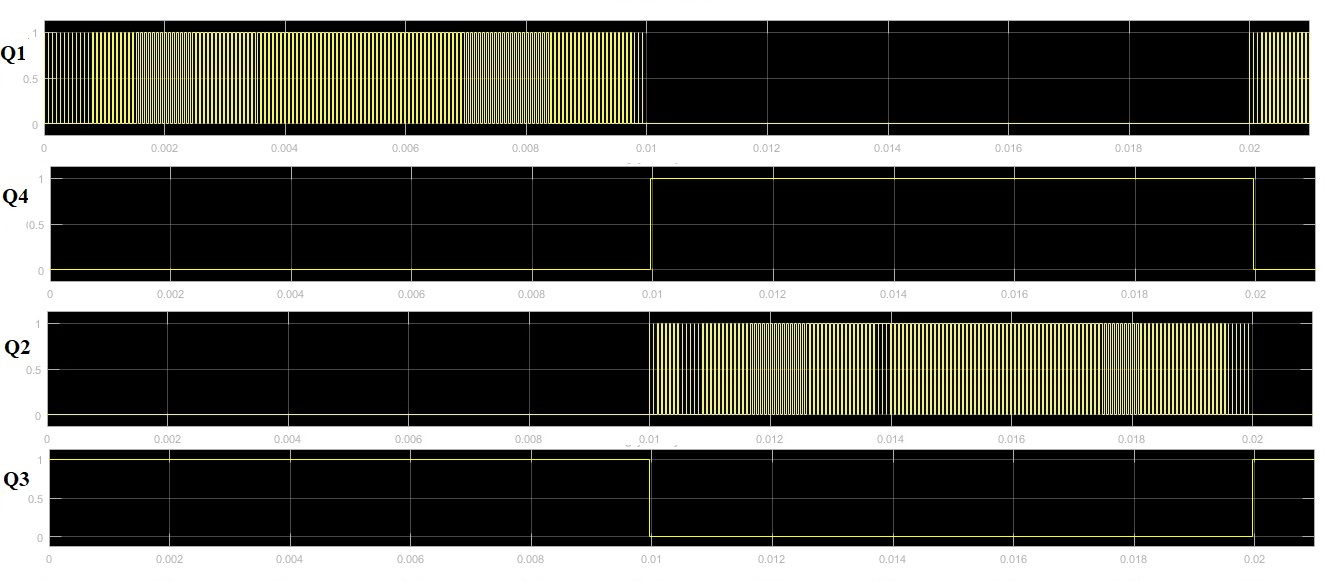
\includegraphics[width=0.98\textwidth]{sistem/onceki_tez_susturma_kapi_darbeleri.jpg}
  \caption{\eskitezetiketi\ Önerilen nötr anahtar susturma yönteminde $Q_1$--$Q_4$ kapı darbelerinin bir temel periyot boyunca görünümü (eski Şekil 4.10).}
  \label{fig:susturma-kapi-darbeleri-tam}
\end{figure}

Şekil~\ref{fig:susturma-kapi-darbeleri-tam} altında pozitif alternansta $Q_1$ anahtarlamayı sürdürürken $Q_4$ komutunun sıfırda tutulduğu; negatif alternansta ise simetrik anahtarlama rolünün karşı kola geçtiği görülmektedir. Şekil~\ref{fig:susturma-kapi-darbeleri-yakin}, yaklaşık \SI{2.2}{\milli\second}--\SI{2.7}{\milli\second} aralığında $Q_1$ darbeleri devam ederken $Q_4$ ve $Q_2$ komutlarının sıfırda, $Q_3$ komutunun iletimde kaldığını daha açık göstermektedir.

\begin{figure}[H]
  \centering
  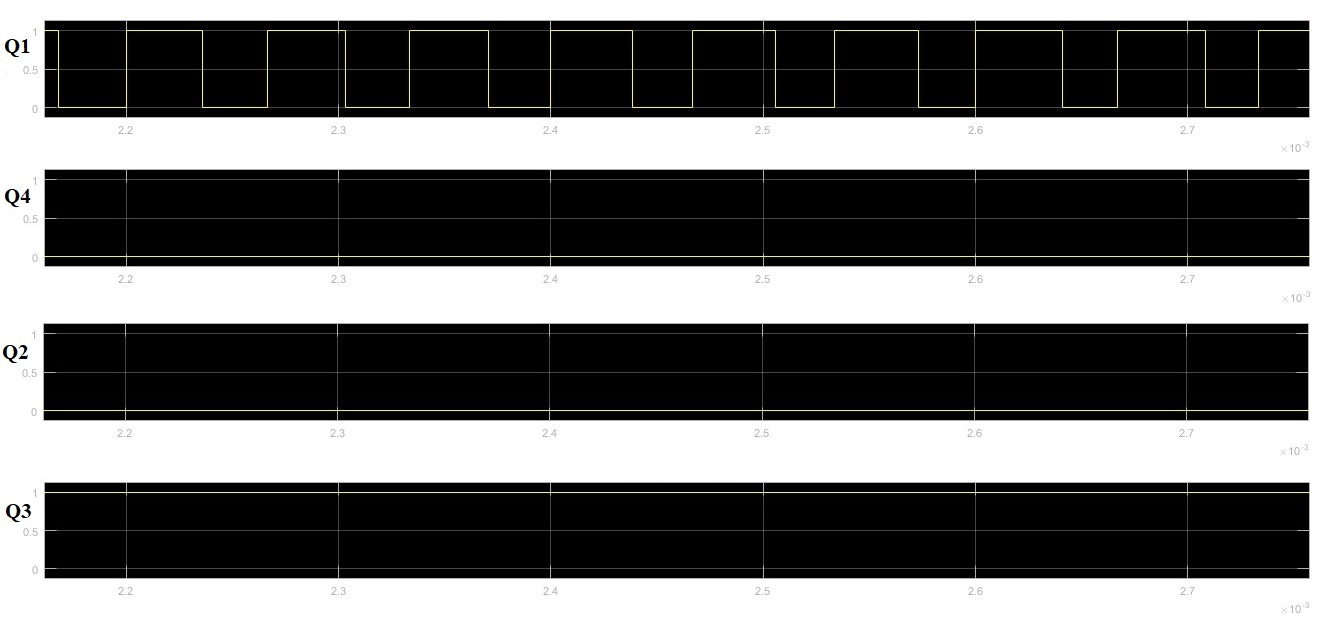
\includegraphics[width=0.98\textwidth]{sistem/onceki_tez_susturma_kapi_darbeleri_yakin.jpg}
  \caption{\eskitezetiketi\ Önerilen nötr anahtar susturma yönteminde seçilmiş anahtarlama penceresinin yakın görünümü (eski Şekil 4.11).}
  \label{fig:susturma-kapi-darbeleri-yakin}
\end{figure}

Şekil~\ref{fig:susturma-l1-tam}, nötr anahtar susturulduğunda $L_1$ akımının sıfırın ters yönünde sürekli dolaşmak yerine her anahtarlama çevriminde sıfıra oturan aralıklar oluşturduğunu göstermektedir. Klasik yöntemin Şekil~\ref{fig:klasik-l1-tam} altındaki iki yönlü dalgalanmasına karşılık burada görülen sıfır-akım aralıkları süreksiz iletim davranışının doğrudan görsel kanıtıdır. Eski Şekil 4.12 başlığında ``büyütülmüş bölüm'' ifadesi kullanılmış olsa da zaman ekseni yaklaşık bir temel periyodu kapsadığından yeni başlık tam-periyot kaydı olarak düzeltilmiştir.

\begin{figure}[H]
  \centering
  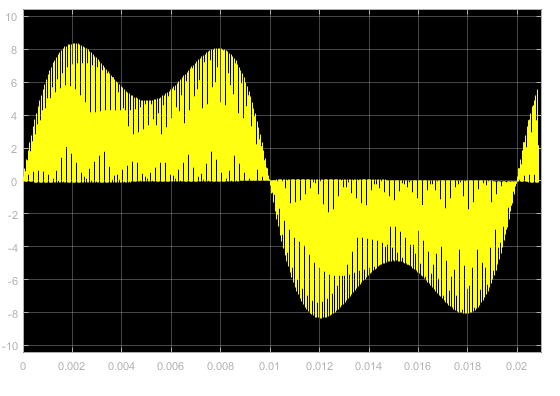
\includegraphics[width=0.82\textwidth]{sonuclar/onceki_tez_susturma_l1_tam.png}
  \caption{\eskitezetiketi\ Nötr anahtar susturma benzetiminde $L_1$ endüktör akımının tam-periyot dalga biçimi (eski Şekil 4.12; başlıktaki ölçek tanımı düzeltilmiştir).}
  \label{fig:susturma-l1-tam}
\end{figure}

Yakın görünüm Şekil~\ref{fig:susturma-l1-yakin} altında verilmiştir. Akımın pozitif eğimle yükselmesinin ardından sıfıra düşmesi ve bir sonraki çevrime kadar sıfırda kalması, nötr kolun klasik senkron serbest dolaşım yolunu sürdürmediğini göstermektedir. Tepe değerinin temel periyot boyunca değişmesi, süreksiz iletim zarfının saf sinüzoidal biçimde kalmadığını da açıklamaktadır.

\begin{figure}[H]
  \centering
  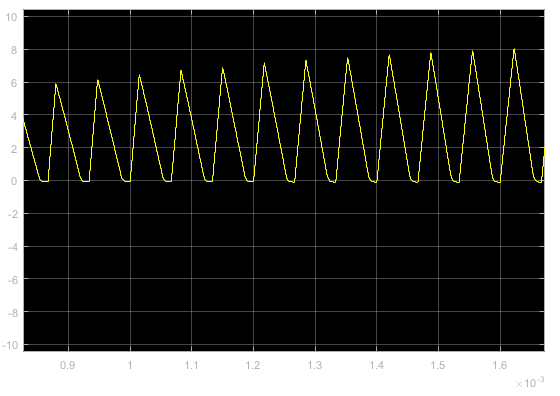
\includegraphics[width=0.82\textwidth]{sonuclar/onceki_tez_susturma_l1_yakin.png}
  \caption{\eskitezetiketi\ Nötr anahtar susturma benzetimindeki $L_1$ endüktör akımından büyütülmüş kesit (eski Şekil 4.13).}
  \label{fig:susturma-l1-yakin}
\end{figure}

Senaryo~2'nin yüksek çözünürlüklü ekranı Şekil~\ref{fig:susturma-dort-kanal} altında dört ölçüm kanalını birlikte göstermektedir. Yukarıdan aşağıya kanallar filtre girişindeki anahtarlamalı gerilim, filtrelenmiş gerilim, $L_1$ endüktör akımı ve LC filtre çıkış akımıdır. Eski başlıkta ikinci kanal ``kontrolör çıkış işareti'' olarak adlandırılmıştır; özgün ekran başlığı gerilim kanalını tanımladığından klasik Senaryo~1'de olduğu gibi burada da kanal adı düzeltilmiştir. $L_1$ ve çıkış akımında görülen düşük frekanslı zarf bozulması, susturmanın tek başına oluşturduğu üçüncü harmonik artışıyla uyumludur.

\begin{figure}[H]
  \centering
  \includegraphics[width=0.98\textwidth]{../dosyalar/05_sonradan_gelenler/Senaryo_2/dalga_sekilleri_s2.jpg}
  \caption{\eskitezetiketi\ Nötr anahtar susturma yönteminde filtre giriş gerilimi, filtrelenmiş gerilim, $L_1$ endüktör akımı ve LC filtre çıkış akımının birlikte gösterimi (eski Şekil 4.14'ün düzeltilmiş kanal açıklaması).}
  \label{fig:susturma-dort-kanal}
\end{figure}

Senaryo~2 FFT ekranlarında analiz başlangıcı \SI{0.06}{\second}, pencere uzunluğu iki çevrim ve temel frekans \SI{50}{\hertz} olarak korunmuştur. Şekil~\ref{fig:susturma-l1-fft} altında $L_1$ akımının temel bileşeni \SI{3.396}{\ampere} ve THD değeri \%46,86; Şekil~\ref{fig:susturma-iout-fft} altında çıkış akımının temel bileşeni \SI{3.412}{\ampere} ve THD değeri \%46,35 olarak okunmaktadır. Filtre çıkışında THD'nin yüksek kalması, bozulmanın yalnız yüksek frekanslı anahtarlama dalgalanmasından değil, filtrenin geçiş bandına daha yakın düşük mertebeli harmoniklerden kaynaklandığını göstermektedir.

\begin{figure}[H]
  \centering
  \includegraphics[width=0.98\textwidth]{../dosyalar/05_sonradan_gelenler/Senaryo_2/THD_IL1.jpg}
  \caption{\eskitezetiketi\ Nötr anahtar susturma yönteminde $L_1$ endüktör akımının FFT analizi: temel bileşen \SI{3.396}{\ampere}, $\mathrm{THD}_{L1}=\%46{,}86$ (eski Şekil 4.15).}
  \label{fig:susturma-l1-fft}
\end{figure}

\begin{figure}[H]
  \centering
  \includegraphics[width=0.98\textwidth]{../dosyalar/05_sonradan_gelenler/Senaryo_2/THD_Iout.jpg}
  \caption{\eskitezetiketi\ Nötr anahtar susturma yönteminde LC filtre çıkış akımının FFT analizi: temel bileşen \SI{3.412}{\ampere}, $\mathrm{THD}_{\mathrm{out}}=\%46{,}35$ (eski Şekil 4.16).}
  \label{fig:susturma-iout-fft}
\end{figure}

Önceki teknik kaynakta T-tipi dönüştürücünün yaklaşık \%7 güçte çalıştırıldığı ayrı bir benzetim için faz akımı THD değeri \%6,1 ve verim \%86,5 olarak raporlanmıştır. İlgili sonucun ham modeli, güç hesabı ve kayıp parametreleri bulunmadığından değerler Senaryo~1--3 tablosuyla birleştirilmemiştir. Tezde yalnız önceki çalışmada raporlanan destekleyici sonuç olarak anılacak, yeni ve yeniden üretilebilir deney sonucu şeklinde kullanılmayacaktır.

\begin{center}
\juriistegietiketi\ \small Düşük, orta ve anma gücü karşılaştırması jüri talebidir. Mevcut arşiv yalnız düşük güç ekranlarını içerdiği için orta ve anma gücü sonuçları Bölüm~\ref{chap:sin3} ve doğrulama bölümünde aday model ile sınırlı, açık bir kanıt statüsü altında verilecektir.
\end{center}

\tezcalismanotu{D4-2 --- Eski Şekil 4.3--4.16'nın ham modelden yeniden üretimi}{Yeni Şekil~4.3--4.16 eski tez ve sonradan gelen ekranlardan ayrı ayrı korunmuştur; ekran görüntüleri çalışma noktası ve dalga biçimi hakkında ikincil kanıttır. Kesin `.slx` ve ham zaman serileri geldiğinde model ekranı, kapı darbeleri, $L_1/I_{out}$ akımları, dört kanallı kayıtlar ve FFT'ler aynı koşu ile ortak analiz penceresinden yeniden üretilecektir. Yeniden üretim başarılı olursa tarihsel rasterların ana metinde kalma, eke taşınma veya çıkarılma kararı verilecektir.}

\tezcalismanotu{D4-3 --- Güç, verim ve THD sayılarındaki tarihsel çelişkiler}{Eski metinde geçen 20~kVA, 25~kW ve yaklaşık 30~kW ifadeleri ile farklı DA bara/faz gerilimleri aynı çalışma noktası kabul edilmeyecektir. Tablo~\ref{tab:onceki-benzetim-ozeti} içindeki verim ve THD değerleri; DA giriş gücü, AA çıkış gücü, işaret yönü, temel/THD analiz penceresi ve kayıp modeli ham kayıttan yeniden hesaplanana kadar tarihsel bulgu statüsünde kalacaktır. Ters akım alanının verim kazancına etkisi, ortak koşullu klasik--susturma karşılaştırması olmadan nedensel üstünlük olarak yazılmayacaktır.}

\section{Bölüm Sonucu}

T-tipi faz kolunun düşük güçte senkron buck benzeri davranışı, nötr kol üzerinden ters enerji dolaşımının fiziksel kaynağını açıklamaktadır. Klasik anahtarlama akım sürekliliği ve THD bakımından avantajlıyken ters akımın RMS ve iletim kayıplarını büyütmesine izin verebilir. Önerilen anahtarlama, ters akımı sürdüren nötr komutunu düşük güç bölgesinde bastırarak kayıp yolunu azaltmayı amaçlamakta; karşılığında süreksiz iletim ve üçüncü harmonik cezası oluşturmaktadır.

Kurtarılan üç benzetim ekranı mekanizma sırasını desteklemektedir. Nötr anahtar susturma çıkış THD değerini \%2,14'ten \%46,35'e yükseltirken Sin\textsuperscript{3} kompanzasyonu değeri \%7,79'a indirmiştir. Ham modelin bulunmaması kapı eşlemesini ve verim iddiasını sınırlandırmaktadır. Sonraki bölümde kompanzasyonun matematiksel tanımı, kapalı çevrim içindeki konumu, Bode analizi ve çalışma noktasına bağlı sonuçları ele alınacaktır.
